%!TEX program = xelatex
\documentclass[8pt, landscape, a4paper]{extarticle}

% --- 核心宏包 ---
\usepackage[UTF8, fontset=fandol]{ctex}
\usepackage[margin=0.8cm, top=1cm, bottom=1.3cm]{geometry}
\usepackage{multicol}
\usepackage{xcolor}
\usepackage{tcolorbox}
\usepackage{enumitem}
\usepackage{amsmath}
\usepackage{amssymb}
\usepackage{fontspec}
\usepackage{tikz}
\usepackage{proof} % 推导规则
\usetikzlibrary{arrows.meta, shapes}

% --- 去掉页码 ---
\pagestyle{empty}

% --- 颜色定义 (Green 主题) ---
\definecolor{headerblue}{RGB}{39, 174, 96}     % Nephritis
\definecolor{navcolor}{RGB}{211, 84, 0}        % 导航橙
\definecolor{intuitioncolor}{RGB}{41, 128, 185}% 直觉蓝
\definecolor{accentcolor}{RGB}{192, 57, 43}    % 强调红
\definecolor{section2}{RGB}{142, 68, 173}      % 紫色
\definecolor{dividergray}{RGB}{220, 220, 220}

% --- 全局设置 ---
\setlength{\parindent}{0pt}
\setlength{\columnsep}{0.4cm} 
\linespread{1.1} 

% --- 列表样式 ---
\setlist[itemize]{leftmargin=1.2em, nosep, itemsep=2pt, topsep=2pt, label=$\textcolor{headerblue}{\vcenter{\hbox{\tiny$\bullet$}}}$ }
\setlist[description]{leftmargin=0.2em, style=sameline, nosep, itemsep=2pt, font=\bfseries}

% --- Box 样式 ---
\newtcolorbox{mybox}[2][]{%
  colback=white,
  colframe=#2,
  coltitle=white,
  boxrule=1pt,             
  arc=2mm,                 
  left=4pt, right=4pt, top=3pt, bottom=3pt, 
  toptitle=3pt, bottomtitle=3pt, 
  fonttitle=\bfseries\sffamily\large,
  title={#1},
  after skip=5pt          
}

% --- 自定义命令 ---
\newcommand{\subt}[1]{{\vspace{2pt}\textbf{\large \textcolor{black}{#1}}}}

\newcommand{\boxdesc}[1]{%
    \textit{\small \textcolor{gray}{#1}}%
    \par\vspace{2pt}%
    {\color{dividergray}\hrule height 0.5pt}%
    \vspace{2pt}%
}

\newcommand{\sepline}{%
    \par \vspace{3pt}%
    {\color{dividergray}\hrule height 0.5pt}%
    \par \vspace{3pt}%
}

% 公式间距
\setlength{\abovedisplayskip}{3pt}
\setlength{\belowdisplayskip}{3pt}

\begin{document}

% --- 页眉 ---
\begin{center}
    {\Huge \textbf{\sffamily \textcolor{headerblue}{类型论 Type Theory Cheat Sheet}}} \\
    \vspace{0.2cm}
    {\large \texttt{Proofs as Programs: The Foundation of Correctness}}
\end{center}

% --- 开始四栏布局 ---
\begin{multicols*}{4}

% === 第一栏 ===

\begin{mybox}[️ 场景导航 (Use Cases)]{navcolor}
    \boxdesc{遇到什么问题 $\to$ 用什么工具}
    \begin{itemize}[itemsep=2pt]
        \item \textbf{编译期查错} $\to$ 静态类型系统
        \item \textbf{形式化验证} $\to$ 依赖类型 (Coq/Agda)
        \item \textbf{泛型编程} $\to$ System F / 多态
        \item \textbf{逻辑证明} $\to$ Curry-Howard 同构
        \item \textbf{内存安全} $\to$ 线性类型 (Rust)
        \item \textbf{自动推导} $\to$ Hindley-Milner 算法
    \end{itemize}
\end{mybox}

\begin{mybox}[1. $\lambda$ 演算 (Lambda Calculus)]{headerblue}
    \boxdesc{计算的原子模型}
    
    \subt{语法}
    $$ e ::= x \mid \lambda x.e \mid e_1 e_2 $$
    \begin{itemize}
        \item \textbf{变量 ($x$)}: 占位符。
        \item \textbf{抽象 ($\lambda x.e$)}: 函数定义。
        \item \textbf{应用 ($e_1 e_2$)}: 函数调用。
    \end{itemize}
    \sepline
    
    \subt{规约 (Reduction)}
    \textbf{$\beta$-规约}: 计算的核心。
    $$ (\lambda x.e) v \longrightarrow e[v/x] $$
    \textit{含义: 把函数体里的 $x$ 替换成参数 $v$。}
    \textbf{$\alpha$-变换}: 变量重命名 ($\lambda x.x \equiv \lambda y.y$)。
\end{mybox}

\begin{mybox}[2. 简单类型 $\lambda$ 演算 (STLC)]{headerblue}
    \boxdesc{给变量贴标签}
    
    \subt{类型 ($\tau$)}
    $$ \tau ::= \text{Bool} \mid \text{Int} \mid \tau_1 \to \tau_2 $$
    \sepline
    
    \subt{定型规则 (Typing Rules)}
    $$ \infer{\Gamma \vdash \lambda x.e : \tau_1 \to \tau_2}{\Gamma, x:\tau_1 \vdash e : \tau_2} $$
    \textit{含义: 如果在假设 $x$ 是 $\tau_1$ 的情况下能推出 $e$ 是 $\tau_2$,那么函数 $\lambda x.e$ 的类型就是 $\tau_1 \to \tau_2$。}
\end{mybox}

\columnbreak

% === 第二栏 ===

\begin{mybox}[3. Curry-Howard 同构]{headerblue}
    \boxdesc{程序 = 证明}
    
    \renewcommand{\arraystretch}{1.2} % 增加行间距
    \vspace{3pt} % 表格上方增加空间
    \begin{tabular}{l|l}
    \textbf{逻辑 (Logic)} & \textbf{编程 (Programming)} \\ \hline
    命题 (Proposition) & 类型 (Type) \\
    证明 (Proof) & 程序 (Program) \\
    蕴含 $P \implies Q$ & 函数 $P \to Q$ \\
    合取 $P \land Q$ & 积类型 $P \times Q$ (Tuple) \\
    析取 $P \lor Q$ & 和类型 $P + Q$ (Union) \\
    全称 $\forall x. P(x)$ & 泛型 / 依赖积 $\Pi$ \\
    存在 $\exists x. P(x)$ & 依赖和 $\Sigma$ \\
    \end{tabular}
    \vspace{3pt} % 表格下方增加空间
    
    \textit{结论: 编写一个通过类型检查的程序,就是证明了一个数学定理。}
\end{mybox}

\begin{mybox}[4. 系统 F (System F)]{headerblue}
    \boxdesc{多态的起源}
    
    \subt{参数多态 (Polymorphism)}
    引入类型变量 $\alpha$。
    $$ \Lambda \alpha. \lambda x:\alpha. x : \forall \alpha. \alpha \to \alpha $$
    \textit{应用: Java/C\# 的 Generics, C++ Templates。}
    \sepline
    
    \subt{Hindley-Milner (HM)}
    System F 的一个受限子集,支持\textbf{完全类型推导}。
    \textit{应用: Haskell, OCaml, Rust (部分)。}
\end{mybox}

\begin{mybox}[5. 依赖类型 (Dependent Types)]{headerblue}
    \boxdesc{类型可以依赖于值}
    
    \subt{定义}
    类型中包含数值。
    \textit{例: \texttt{Vec<Int, 3>} (长度为3的数组)。}
    $$ \Pi (x:A). B(x) $$
    返回值的类型 $B$ 取决于输入参数 $x$ 的值。
    \sepline
    
    \subt{应用}
    消除数组越界错误。
    证明排序算法的输出确实是有序的。
    \textit{语言: Idris, Agda, Coq, Lean。}
    \sepline
    
    \subt{精制类型 (Refinement Types)}
    基础类型 + 谓词。$\{x: \text{Int} \mid x > 0\}$。
\end{mybox}

\columnbreak

% === 第三栏 ===

\begin{mybox}[6. 线性类型 (Linear Types)]{headerblue}
    \boxdesc{资源管理}
    
    \subt{规则}
    每个变量\textbf{必须}且\textbf{只能}被使用一次。
    \sepline
    
    \subt{应用}
    \begin{itemize}
        \item \textbf{内存管理}: Rust 的 Ownership/Borrowing 机制深受其影响。
        \item \textbf{量子计算}: 量子态不能被复制 (No-cloning)。
        \item \textbf{并发编程}: Session Types 保证通信协议正确。
    \end{itemize}
    \sepline
    
    \subt{变体}
    \textbf{仿射类型}: 最多一次。 \textbf{相关类型}: 至少一次。
\end{mybox}

\begin{mybox}[7. 常见类型系统特性]{headerblue}
    \boxdesc{术语表}
    \begin{itemize}
        \item \textbf{协变 (Covariance)}: 子类数组是父类数组。
        \item \textbf{逆变 (Contravariance)}: 函数参数类型相反。
        \item \textbf{结构化类型 (Duck Typing)}: 长得像就是。
        \item \textbf{名义类型 (Nominal)}: 名字一样才是。
        \item \textbf{子类型 (Subtyping)}: $S <: T$,S 可用在 T 处。
    \end{itemize}
\end{mybox}

\begin{mybox}[8. 同伦类型论 (HoTT)]{headerblue}
    \boxdesc{数学的新基础}
    
    \subt{Univalence Axiom}
    等价的类型是相等的。
    $$ (A \simeq B) \simeq (A = B) $$
    把拓扑学中的“路径”概念引入类型论。
    \textit{类型是空间,程序是路径。}
    \sepline
    
    \subt{立方类型论 (Cubical Type Theory)}
    HoTT 的计算性解释。
    \textit{使得单价公理具有计算意义,可用于编程。}
    $$ \text{Path } A \ a \ b $$
    \sepline
    
    \subt{高阶归纳类型 (HITs)}
    不仅定义点,还定义路径。
    \textit{例: 圆 $S^1$ 由基点 base 和路径 loop 构成。}
\end{mybox}

\columnbreak

% === 第四栏 ===

\begin{mybox}[9. 实践中的类型]{headerblue}
    \boxdesc{TypeScript / Rust}
    
    \subt{代数数据类型 (ADT)}
    \begin{itemize}
        \item \textbf{Sum}: \texttt{enum Option \{ Some(T), None \}}
        \item \textbf{Product}: \texttt{struct Point \{ x: i32, y: i32 \}}
    \end{itemize}
    \sepline
    
    \subt{模式匹配 (Pattern Matching)}
    解构 ADT 的利器。
    \texttt{match val \{ Some(x) => ..., None => ... \}}
    \textit{编译器检查穷尽性 (Exhaustiveness Check)。}
    \sepline
    
    \subt{类型推导 (Type Inference)}
    编译器自动推断类型。
    \texttt{let x = 10;} // 自动推断为 int
    \sepline
    
    \subt{高阶类型 (HKT)}
    类型构造器的类型。
    \textit{例: \texttt{Monad m} 中的 \texttt{m} 是 \texttt{* -> *}。}
\end{mybox}

\vspace*{\fill}

\begin{mybox}[ 核心直觉 (Intuition)]{intuitioncolor}
    \boxdesc{“类型是程序的守门人。”}
    
    % TikZ 矢量图: 推导树 (Derivation Tree)
    \begin{center}
    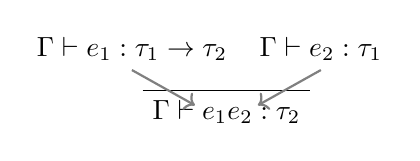
\begin{tikzpicture}[scale=0.8]
        \node (bot) at (0,0) {$\Gamma \vdash e_1 e_2 : \tau_2$};
        \node (left) at (-1.5, 1) {$\Gamma \vdash e_1 : \tau_1 \to \tau_2$};
        \node (right) at (1.5, 1) {$\Gamma \vdash e_2 : \tau_1$};
        
        \draw (bot.north west) -- (bot.north east);
        \draw[->, thick, gray] (left.south) -- (-0.5, 0.1);
        \draw[->, thick, gray] (right.south) -- (0.5, 0.1);
    \end{tikzpicture}
    \end{center}

    \hspace{1em}类型不仅仅是用来查错的,它是\textbf{设计文档},是\textbf{逻辑规范}。
    \vspace{4pt}
    
    \subt{三大核心视角}
    \begin{itemize}[itemsep=4pt]
        \item \textbf{良构即正确}: 
        "Well-typed programs cannot go wrong." (Milner)。类型系统保证了程序在运行时不会发生某些特定的错误 (如把整数当函数调用)。
        
        \item \textbf{类型驱动开发 (TDD)}: 
        先写函数签名 (类型),再写实现。让编译器指导你补全代码 (Type Holes)。
        
        \item \textbf{表达力 vs 可判定性}: 
        类型系统越强大 (如依赖类型),能证明的定理越多,但编译器的自动推导越难,甚至不可判定 (图灵停机问题)。
    \end{itemize}
    
    \vspace{6pt}
    \centering\textit{\footnotesize 动态类型是一时之爽,静态类型是一世之安。}
\end{mybox}

\end{multicols*}

\end{document}
